\documentclass{standalone}
\usepackage{tikz}
\usetikzlibrary{patterns, positioning}
\usepackage[sfdefault]{ClearSans} %% option 'sfdefault' activates Clear Sans as the default text font
\usepackage[T1]{fontenc}

\begin{document}
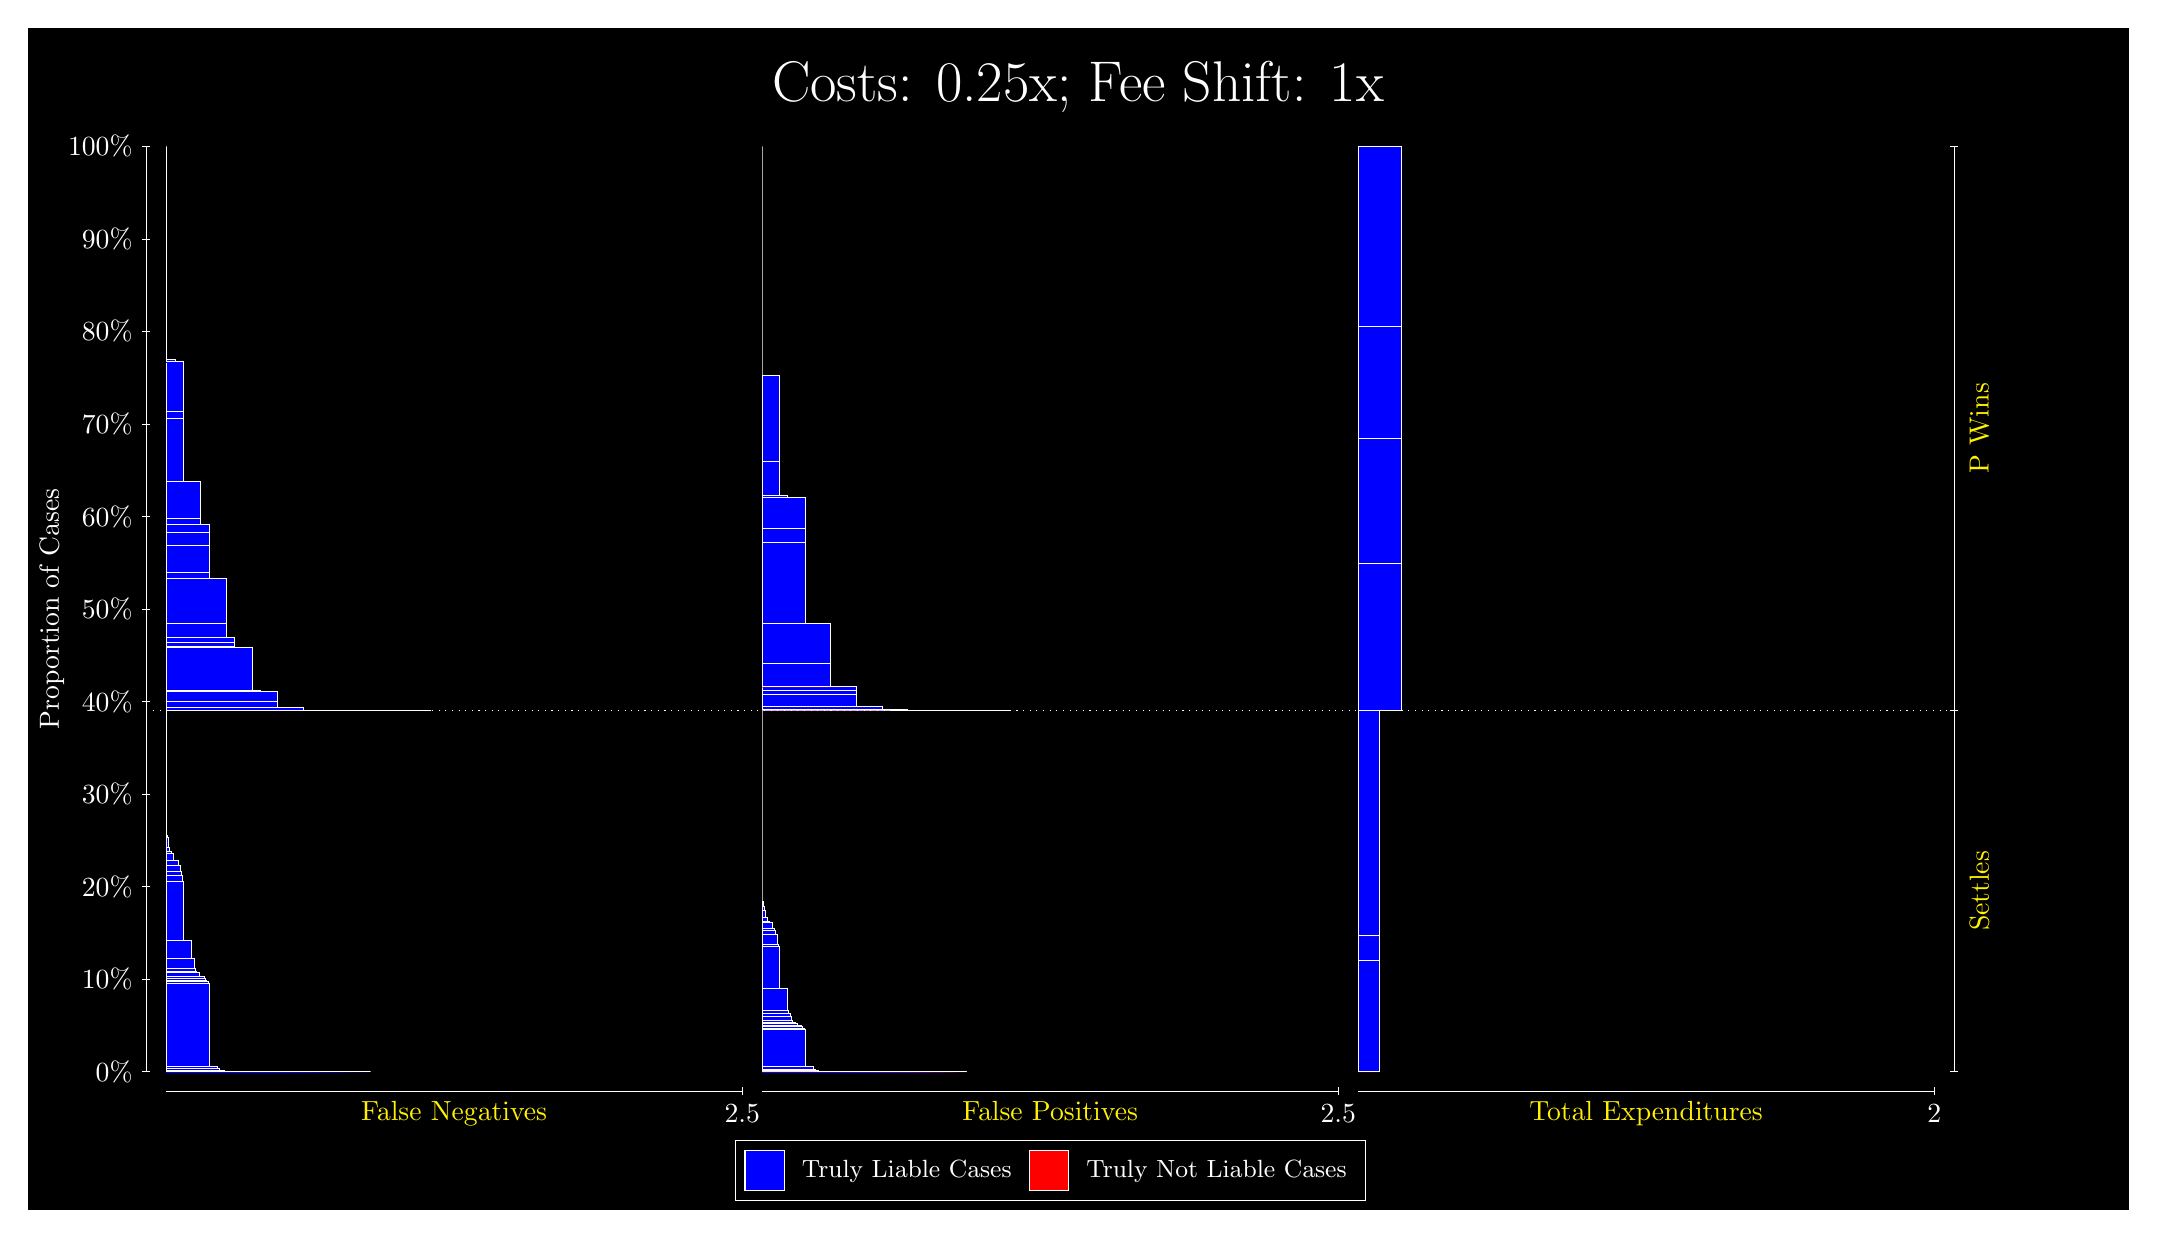
\begin{tikzpicture}
\draw[fill=black] (0,0) rectangle (26.667,15);
\draw[text=white] (0,13.5) rectangle (26.667,15) node[midway] {\huge Costs: 0.25x; Fee Shift: 1x};
\draw[white, very thin] (1.5,1.75) -- (1.5,13.5);
\node[rotate=90, text=white, anchor=center] at (0.3, 7.625) {Proportion of Cases};
\draw[white, very thin] (1.45,1.75) -- (1.55,1.75);
\node[text=white, anchor=east] at (1.45, 1.75) {0\%};
\draw[white, very thin] (1.45,2.925) -- (1.55,2.925);
\node[text=white, anchor=east] at (1.45, 2.925) {10\%};
\draw[white, very thin] (1.45,4.1) -- (1.55,4.1);
\node[text=white, anchor=east] at (1.45, 4.1) {20\%};
\draw[white, very thin] (1.45,5.275) -- (1.55,5.275);
\node[text=white, anchor=east] at (1.45, 5.275) {30\%};
\draw[white, very thin] (1.45,6.45) -- (1.55,6.45);
\node[text=white, anchor=east] at (1.45, 6.45) {40\%};
\draw[white, very thin] (1.45,7.625) -- (1.55,7.625);
\node[text=white, anchor=east] at (1.45, 7.625) {50\%};
\draw[white, very thin] (1.45,8.8) -- (1.55,8.8);
\node[text=white, anchor=east] at (1.45, 8.8) {60\%};
\draw[white, very thin] (1.45,9.975) -- (1.55,9.975);
\node[text=white, anchor=east] at (1.45, 9.975) {70\%};
\draw[white, very thin] (1.45,11.15) -- (1.55,11.15);
\node[text=white, anchor=east] at (1.45, 11.15) {80\%};
\draw[white, very thin] (1.45,12.325) -- (1.55,12.325);
\node[text=white, anchor=east] at (1.45, 12.325) {90\%};
\draw[white, very thin] (1.45,13.5) -- (1.55,13.5);
\node[text=white, anchor=east] at (1.45, 13.5) {100\%};

\draw[white, very thin] (24.457,1.75) -- (24.457,13.5);
\draw[white, very thin] (24.407,1.75) -- (24.507,1.75);
\node[anchor=west] at (24.407, 1.75) {};
\draw[white, very thin] (24.407,6.3386) -- (24.507,6.3386);
\node[anchor=west] at (24.407, 6.3386) {};
\draw[white, very thin] (24.407,13.5) -- (24.507,13.5);
\node[anchor=west] at (24.407, 13.5) {};

\draw[white, very thin, fill=blue] (1.75,1.75) rectangle (4.3482,1.75);
\draw[white, very thin, fill=blue] (1.75,1.75) rectangle (4.2018,1.75);
\draw[white, very thin, fill=blue] (1.75,1.75) rectangle (4.0554,1.75);
\draw[white, very thin, fill=blue] (1.75,1.75) rectangle (4.0229,1.75);
\draw[white, very thin, fill=blue] (1.75,1.75) rectangle (3.9091,1.75);
\draw[white, very thin, fill=blue] (1.75,1.75) rectangle (3.8765,1.75);
\draw[white, very thin, fill=blue] (1.75,1.75) rectangle (3.7627,1.75);
\draw[white, very thin, fill=blue] (1.75,1.75) rectangle (3.7302,1.75);
\draw[white, very thin, fill=blue] (1.75,1.75) rectangle (3.6976,1.75);
\draw[white, very thin, fill=blue] (1.75,1.75) rectangle (3.6163,1.75);
\draw[white, very thin, fill=blue] (1.75,1.75) rectangle (3.5838,1.75);
\draw[white, very thin, fill=blue] (1.75,1.75) rectangle (3.5513,1.75);
\draw[white, very thin, fill=blue] (1.75,1.75) rectangle (3.4699,1.75);
\draw[white, very thin, fill=blue] (1.75,1.75) rectangle (3.4374,1.75);
\draw[white, very thin, fill=blue] (1.75,1.75) rectangle (3.4049,1.75);
\draw[white, very thin, fill=blue] (1.75,1.75) rectangle (3.3723,1.75);
\draw[white, very thin, fill=blue] (1.75,1.75) rectangle (3.3236,1.75);
\draw[white, very thin, fill=blue] (1.75,1.75) rectangle (3.291,1.75);
\draw[white, very thin, fill=blue] (1.75,1.75) rectangle (3.2585,1.75);
\draw[white, very thin, fill=blue] (1.75,1.75) rectangle (3.226,1.75);
\draw[white, very thin, fill=blue] (1.75,1.75) rectangle (3.1772,1.75);
\draw[white, very thin, fill=blue] (1.75,1.75) rectangle (3.1447,1.75);
\draw[white, very thin, fill=blue] (1.75,1.75) rectangle (3.1121,1.75);
\draw[white, very thin, fill=blue] (1.75,1.75) rectangle (3.0796,1.75);
\draw[white, very thin, fill=blue] (1.75,1.75) rectangle (3.0471,1.75);
\draw[white, very thin, fill=blue] (1.75,1.75) rectangle (3.0308,1.75);
\draw[white, very thin, fill=blue] (1.75,1.75) rectangle (2.9983,1.75);
\draw[white, very thin, fill=blue] (1.75,1.75) rectangle (2.9657,1.75);
\draw[white, very thin, fill=blue] (1.75,1.75) rectangle (2.9332,1.75);
\draw[white, very thin, fill=blue] (1.75,1.75) rectangle (2.9007,1.75);
\draw[white, very thin, fill=blue] (1.75,1.75) rectangle (2.8844,1.7501);
\draw[white, very thin, fill=blue] (1.75,1.7501) rectangle (2.8519,1.7501);
\draw[white, very thin, fill=blue] (1.75,1.7501) rectangle (2.8194,1.7501);
\draw[white, very thin, fill=blue] (1.75,1.7501) rectangle (2.7868,1.7503);
\draw[white, very thin, fill=blue] (1.75,1.7503) rectangle (2.7543,1.7508);
\draw[white, very thin, fill=blue] (1.75,1.7508) rectangle (2.738,1.7508);
\draw[white, very thin, fill=blue] (1.75,1.7508) rectangle (2.7218,1.7513);
\draw[white, very thin, fill=blue] (1.75,1.7513) rectangle (2.7055,1.7513);
\draw[white, very thin, fill=blue] (1.75,1.7513) rectangle (2.673,1.7513);
\draw[white, very thin, fill=blue] (1.75,1.7513) rectangle (2.6405,1.7513);
\draw[white, very thin, fill=blue] (1.75,1.7513) rectangle (2.6079,1.7532);
\draw[white, very thin, fill=blue] (1.75,1.7532) rectangle (2.5917,1.7537);
\draw[white, very thin, fill=blue] (1.75,1.7537) rectangle (2.5754,1.7554);
\draw[white, very thin, fill=blue] (1.75,1.7554) rectangle (2.5591,1.7569);
\draw[white, very thin, fill=blue] (1.75,1.7569) rectangle (2.5266,1.7569);
\draw[white, very thin, fill=blue] (1.75,1.7569) rectangle (2.4941,1.7614);
\draw[white, very thin, fill=blue] (1.75,1.7614) rectangle (2.4616,1.7658);
\draw[white, very thin, fill=blue] (1.75,1.7658) rectangle (2.4453,1.771);
\draw[white, very thin, fill=blue] (1.75,1.771) rectangle (2.429,1.791);
\draw[white, very thin, fill=blue] (1.75,1.791) rectangle (2.4128,1.7917);
\draw[white, very thin, fill=blue] (1.75,1.7917) rectangle (2.3965,1.8153);
\draw[white, very thin, fill=blue] (1.75,1.8153) rectangle (2.3802,1.8153);
\draw[white, very thin, fill=blue] (1.75,1.8153) rectangle (2.3477,1.8154);
\draw[white, very thin, fill=blue] (1.75,1.8154) rectangle (2.3152,1.8154);
\draw[white, very thin, fill=blue] (1.75,1.8154) rectangle (2.2989,2.8712);
\draw[white, very thin, fill=blue] (1.75,2.8712) rectangle (2.2827,2.9007);
\draw[white, very thin, fill=blue] (1.75,2.9007) rectangle (2.2664,2.9094);
\draw[white, very thin, fill=blue] (1.75,2.9094) rectangle (2.2501,2.9393);
\draw[white, very thin, fill=blue] (1.75,2.9393) rectangle (2.2339,2.9606);
\draw[white, very thin, fill=blue] (1.75,2.9606) rectangle (2.2013,2.9618);
\draw[white, very thin, fill=blue] (1.75,2.9618) rectangle (2.1688,3.0066);
\draw[white, very thin, fill=blue] (1.75,3.0066) rectangle (2.1363,3.0281);
\draw[white, very thin, fill=blue] (1.75,3.0281) rectangle (2.12,3.0574);
\draw[white, very thin, fill=blue] (1.75,3.0574) rectangle (2.1037,3.1852);
\draw[white, very thin, fill=blue] (1.75,3.1852) rectangle (2.0875,3.1944);
\draw[white, very thin, fill=blue] (1.75,3.1944) rectangle (2.0712,3.419);
\draw[white, very thin, fill=blue] (1.75,3.419) rectangle (2.055,3.4196);
\draw[white, very thin, fill=blue] (1.75,3.4196) rectangle (2.0224,3.4197);
\draw[white, very thin, fill=blue] (1.75,3.4197) rectangle (1.9899,3.4197);
\draw[white, very thin, fill=blue] (1.75,3.4197) rectangle (1.9736,4.1717);
\draw[white, very thin, fill=blue] (1.75,4.1717) rectangle (1.9574,4.2456);
\draw[white, very thin, fill=blue] (1.75,4.2456) rectangle (1.9411,4.2887);
\draw[white, very thin, fill=blue] (1.75,4.2887) rectangle (1.9248,4.3756);
\draw[white, very thin, fill=blue] (1.75,4.3756) rectangle (1.9086,4.436);
\draw[white, very thin, fill=blue] (1.75,4.436) rectangle (1.876,4.439);
\draw[white, very thin, fill=blue] (1.75,4.439) rectangle (1.8435,4.5252);
\draw[white, very thin, fill=blue] (1.75,4.5252) rectangle (1.811,4.5441);
\draw[white, very thin, fill=blue] (1.75,4.5441) rectangle (1.7947,4.5941);
\draw[white, very thin, fill=blue] (1.75,4.5941) rectangle (1.7785,4.726);
\draw[white, very thin, fill=blue] (1.75,4.726) rectangle (1.7622,4.7521);
\draw[white, very thin, fill=red] (1.75,4.7521) rectangle (1.75,4.7521);
\draw[white, very thin, fill=blue] (1.75,4.7521) rectangle (1.75,6.3386);
\draw[white, very thin, fill=blue] (1.75,6.3386) rectangle (5.1167,6.3386);
\draw[white, very thin, fill=blue] (1.75,6.3386) rectangle (4.7914,6.3386);
\draw[white, very thin, fill=blue] (1.75,6.3386) rectangle (4.7914,6.3386);
\draw[white, very thin, fill=blue] (1.75,6.3386) rectangle (4.5718,6.3386);
\draw[white, very thin, fill=blue] (1.75,6.3386) rectangle (4.4661,6.3386);
\draw[white, very thin, fill=blue] (1.75,6.3386) rectangle (4.4661,6.3387);
\draw[white, very thin, fill=blue] (1.75,6.3387) rectangle (4.2465,6.3387);
\draw[white, very thin, fill=blue] (1.75,6.3387) rectangle (4.2465,6.3387);
\draw[white, very thin, fill=blue] (1.75,6.3387) rectangle (4.1408,6.3389);
\draw[white, very thin, fill=blue] (1.75,6.3389) rectangle (3.9213,6.3389);
\draw[white, very thin, fill=blue] (1.75,6.3389) rectangle (3.8155,6.3414);
\draw[white, very thin, fill=blue] (1.75,6.3414) rectangle (3.8155,6.3432);
\draw[white, very thin, fill=blue] (1.75,6.3432) rectangle (3.596,6.3432);
\draw[white, very thin, fill=blue] (1.75,6.3432) rectangle (3.4903,6.3813);
\draw[white, very thin, fill=blue] (1.75,6.3813) rectangle (3.2707,6.3813);
\draw[white, very thin, fill=blue] (1.75,6.3813) rectangle (3.2707,6.3814);
\draw[white, very thin, fill=blue] (1.75,6.3814) rectangle (3.165,6.4538);
\draw[white, very thin, fill=blue] (1.75,6.4538) rectangle (3.165,6.5766);
\draw[white, very thin, fill=blue] (1.75,6.5766) rectangle (2.9454,6.5772);
\draw[white, very thin, fill=blue] (1.75,6.5772) rectangle (2.9454,6.5824);
\draw[white, very thin, fill=blue] (1.75,6.5824) rectangle (2.9454,6.5862);
\draw[white, very thin, fill=blue] (1.75,6.5862) rectangle (2.8397,7.137);
\draw[white, very thin, fill=blue] (1.75,7.137) rectangle (2.6201,7.1457);
\draw[white, very thin, fill=blue] (1.75,7.1457) rectangle (2.6201,7.2064);
\draw[white, very thin, fill=blue] (1.75,7.2064) rectangle (2.6201,7.2652);
\draw[white, very thin, fill=blue] (1.75,7.2652) rectangle (2.5144,7.4378);
\draw[white, very thin, fill=blue] (1.75,7.4378) rectangle (2.5144,8.0107);
\draw[white, very thin, fill=blue] (1.75,8.0107) rectangle (2.2948,8.0868);
\draw[white, very thin, fill=blue] (1.75,8.0868) rectangle (2.2948,8.431);
\draw[white, very thin, fill=blue] (1.75,8.431) rectangle (2.2948,8.603);
\draw[white, very thin, fill=blue] (1.75,8.603) rectangle (2.2948,8.6989);
\draw[white, very thin, fill=blue] (1.75,8.6989) rectangle (2.1891,8.7789);
\draw[white, very thin, fill=blue] (1.75,8.7789) rectangle (2.1891,9.2403);
\draw[white, very thin, fill=blue] (1.75,9.2403) rectangle (1.9696,10.045);
\draw[white, very thin, fill=blue] (1.75,10.045) rectangle (1.9696,10.14);
\draw[white, very thin, fill=blue] (1.75,10.14) rectangle (1.9696,10.765);
\draw[white, very thin, fill=blue] (1.75,10.765) rectangle (1.8638,10.766);
\draw[white, very thin, fill=blue] (1.75,10.766) rectangle (1.8638,10.771);
\draw[white, very thin, fill=blue] (1.75,10.771) rectangle (1.8638,10.794);
\draw[white, very thin, fill=blue] (1.75,10.794) rectangle (1.8638,10.794);
\draw[white, very thin, fill=red] (1.75,10.794) rectangle (1.75,10.794);
\draw[white, very thin, fill=blue] (1.75,10.794) rectangle (1.75,13.5);
\draw[white, very thin, fill=red] (9.3189,1.75) rectangle (11.917,1.75);
\draw[white, very thin, fill=blue] (9.3189,1.75) rectangle (11.917,1.75);
\draw[white, very thin, fill=red] (9.3189,1.75) rectangle (11.771,1.75);
\draw[white, very thin, fill=blue] (9.3189,1.75) rectangle (11.771,1.75);
\draw[white, very thin, fill=red] (9.3189,1.75) rectangle (11.624,1.75);
\draw[white, very thin, fill=blue] (9.3189,1.75) rectangle (11.624,1.75);
\draw[white, very thin, fill=blue] (9.3189,1.75) rectangle (11.592,1.75);
\draw[white, very thin, fill=red] (9.3189,1.75) rectangle (11.478,1.75);
\draw[white, very thin, fill=blue] (9.3189,1.75) rectangle (11.478,1.75);
\draw[white, very thin, fill=blue] (9.3189,1.75) rectangle (11.445,1.75);
\draw[white, very thin, fill=red] (9.3189,1.75) rectangle (11.332,1.75);
\draw[white, very thin, fill=blue] (9.3189,1.75) rectangle (11.332,1.75);
\draw[white, very thin, fill=blue] (9.3189,1.75) rectangle (11.299,1.75);
\draw[white, very thin, fill=blue] (9.3189,1.75) rectangle (11.266,1.75);
\draw[white, very thin, fill=red] (9.3189,1.75) rectangle (11.185,1.75);
\draw[white, very thin, fill=blue] (9.3189,1.75) rectangle (11.185,1.75);
\draw[white, very thin, fill=blue] (9.3189,1.75) rectangle (11.153,1.75);
\draw[white, very thin, fill=blue] (9.3189,1.75) rectangle (11.12,1.75);
\draw[white, very thin, fill=red] (9.3189,1.75) rectangle (11.039,1.75);
\draw[white, very thin, fill=blue] (9.3189,1.75) rectangle (11.039,1.75);
\draw[white, very thin, fill=blue] (9.3189,1.75) rectangle (11.006,1.75);
\draw[white, very thin, fill=blue] (9.3189,1.75) rectangle (10.974,1.75);
\draw[white, very thin, fill=blue] (9.3189,1.75) rectangle (10.941,1.75);
\draw[white, very thin, fill=red] (9.3189,1.75) rectangle (10.892,1.75);
\draw[white, very thin, fill=blue] (9.3189,1.75) rectangle (10.892,1.75);
\draw[white, very thin, fill=blue] (9.3189,1.75) rectangle (10.86,1.75);
\draw[white, very thin, fill=blue] (9.3189,1.75) rectangle (10.827,1.75);
\draw[white, very thin, fill=blue] (9.3189,1.75) rectangle (10.795,1.75);
\draw[white, very thin, fill=red] (9.3189,1.75) rectangle (10.746,1.75);
\draw[white, very thin, fill=blue] (9.3189,1.75) rectangle (10.746,1.75);
\draw[white, very thin, fill=blue] (9.3189,1.75) rectangle (10.714,1.75);
\draw[white, very thin, fill=blue] (9.3189,1.75) rectangle (10.681,1.75);
\draw[white, very thin, fill=blue] (9.3189,1.75) rectangle (10.648,1.75);
\draw[white, very thin, fill=blue] (9.3189,1.75) rectangle (10.616,1.75);
\draw[white, very thin, fill=red] (9.3189,1.75) rectangle (10.6,1.75);
\draw[white, very thin, fill=blue] (9.3189,1.75) rectangle (10.6,1.75);
\draw[white, very thin, fill=blue] (9.3189,1.75) rectangle (10.567,1.75);
\draw[white, very thin, fill=blue] (9.3189,1.75) rectangle (10.535,1.75);
\draw[white, very thin, fill=blue] (9.3189,1.75) rectangle (10.502,1.75);
\draw[white, very thin, fill=blue] (9.3189,1.75) rectangle (10.47,1.75);
\draw[white, very thin, fill=red] (9.3189,1.75) rectangle (10.453,1.75);
\draw[white, very thin, fill=blue] (9.3189,1.75) rectangle (10.453,1.75);
\draw[white, very thin, fill=blue] (9.3189,1.75) rectangle (10.421,1.7501);
\draw[white, very thin, fill=blue] (9.3189,1.7501) rectangle (10.388,1.7501);
\draw[white, very thin, fill=blue] (9.3189,1.7501) rectangle (10.356,1.7501);
\draw[white, very thin, fill=blue] (9.3189,1.7501) rectangle (10.323,1.7504);
\draw[white, very thin, fill=red] (9.3189,1.7504) rectangle (10.307,1.7504);
\draw[white, very thin, fill=blue] (9.3189,1.7504) rectangle (10.307,1.7504);
\draw[white, very thin, fill=blue] (9.3189,1.7504) rectangle (10.291,1.7516);
\draw[white, very thin, fill=blue] (9.3189,1.7516) rectangle (10.274,1.7516);
\draw[white, very thin, fill=blue] (9.3189,1.7516) rectangle (10.242,1.7516);
\draw[white, very thin, fill=blue] (9.3189,1.7516) rectangle (10.209,1.7517);
\draw[white, very thin, fill=blue] (9.3189,1.7517) rectangle (10.177,1.753);
\draw[white, very thin, fill=red] (9.3189,1.753) rectangle (10.161,1.753);
\draw[white, very thin, fill=blue] (9.3189,1.753) rectangle (10.161,1.7542);
\draw[white, very thin, fill=blue] (9.3189,1.7542) rectangle (10.144,1.7553);
\draw[white, very thin, fill=blue] (9.3189,1.7553) rectangle (10.128,1.7553);
\draw[white, very thin, fill=blue] (9.3189,1.7553) rectangle (10.095,1.7571);
\draw[white, very thin, fill=blue] (9.3189,1.7571) rectangle (10.063,1.7572);
\draw[white, very thin, fill=blue] (9.3189,1.7572) rectangle (10.03,1.7603);
\draw[white, very thin, fill=red] (9.3189,1.7603) rectangle (10.014,1.7603);
\draw[white, very thin, fill=blue] (9.3189,1.7603) rectangle (10.014,1.7695);
\draw[white, very thin, fill=blue] (9.3189,1.7695) rectangle (9.9979,1.777);
\draw[white, very thin, fill=blue] (9.3189,1.777) rectangle (9.9816,1.7792);
\draw[white, very thin, fill=blue] (9.3189,1.7792) rectangle (9.9654,1.8161);
\draw[white, very thin, fill=blue] (9.3189,1.8161) rectangle (9.9491,1.8161);
\draw[white, very thin, fill=blue] (9.3189,1.8161) rectangle (9.9166,1.8161);
\draw[white, very thin, fill=blue] (9.3189,1.8161) rectangle (9.884,1.8166);
\draw[white, very thin, fill=red] (9.3189,1.8166) rectangle (9.8678,1.8166);
\draw[white, very thin, fill=blue] (9.3189,1.8166) rectangle (9.8678,2.2807);
\draw[white, very thin, fill=blue] (9.3189,2.2807) rectangle (9.8515,2.2942);
\draw[white, very thin, fill=blue] (9.3189,2.2942) rectangle (9.8353,2.319);
\draw[white, very thin, fill=blue] (9.3189,2.319) rectangle (9.819,2.3362);
\draw[white, very thin, fill=blue] (9.3189,2.3362) rectangle (9.8027,2.339);
\draw[white, very thin, fill=blue] (9.3189,2.339) rectangle (9.7702,2.3691);
\draw[white, very thin, fill=blue] (9.3189,2.3691) rectangle (9.7377,2.3703);
\draw[white, very thin, fill=blue] (9.3189,2.3703) rectangle (9.7051,2.4017);
\draw[white, very thin, fill=blue] (9.3189,2.4017) rectangle (9.6889,2.4528);
\draw[white, very thin, fill=blue] (9.3189,2.4528) rectangle (9.6726,2.4954);
\draw[white, very thin, fill=blue] (9.3189,2.4954) rectangle (9.6563,2.5252);
\draw[white, very thin, fill=blue] (9.3189,2.5252) rectangle (9.6401,2.8087);
\draw[white, very thin, fill=blue] (9.3189,2.8087) rectangle (9.6238,2.8087);
\draw[white, very thin, fill=blue] (9.3189,2.8087) rectangle (9.5913,2.8088);
\draw[white, very thin, fill=blue] (9.3189,2.8088) rectangle (9.5588,2.8101);
\draw[white, very thin, fill=blue] (9.3189,2.8101) rectangle (9.5425,3.3366);
\draw[white, very thin, fill=blue] (9.3189,3.3366) rectangle (9.5262,3.3626);
\draw[white, very thin, fill=blue] (9.3189,3.3626) rectangle (9.51,3.4945);
\draw[white, very thin, fill=blue] (9.3189,3.4945) rectangle (9.4937,3.5445);
\draw[white, very thin, fill=blue] (9.3189,3.5445) rectangle (9.4774,3.5634);
\draw[white, very thin, fill=blue] (9.3189,3.5634) rectangle (9.4449,3.6496);
\draw[white, very thin, fill=blue] (9.3189,3.6496) rectangle (9.4124,3.6527);
\draw[white, very thin, fill=blue] (9.3189,3.6527) rectangle (9.3799,3.713);
\draw[white, very thin, fill=blue] (9.3189,3.713) rectangle (9.3636,3.8);
\draw[white, very thin, fill=blue] (9.3189,3.8) rectangle (9.3473,3.8431);
\draw[white, very thin, fill=blue] (9.3189,3.8431) rectangle (9.3311,3.917);
\draw[white, very thin, fill=blue] (9.3189,3.917) rectangle (9.3189,6.3386);
\draw[white, very thin, fill=red] (9.3189,6.3386) rectangle (12.466,6.3386);
\draw[white, very thin, fill=blue] (9.3189,6.3386) rectangle (12.466,6.3386);
\draw[white, very thin, fill=red] (9.3189,6.3386) rectangle (12.141,6.3386);
\draw[white, very thin, fill=blue] (9.3189,6.3386) rectangle (12.141,6.3386);
\draw[white, very thin, fill=red] (9.3189,6.3386) rectangle (11.815,6.3386);
\draw[white, very thin, fill=blue] (9.3189,6.3386) rectangle (11.815,6.3387);
\draw[white, very thin, fill=blue] (9.3189,6.3387) rectangle (11.815,6.3387);
\draw[white, very thin, fill=blue] (9.3189,6.3387) rectangle (11.49,6.3388);
\draw[white, very thin, fill=red] (9.3189,6.3388) rectangle (11.49,6.3388);
\draw[white, very thin, fill=blue] (9.3189,6.3388) rectangle (11.49,6.3391);
\draw[white, very thin, fill=red] (9.3189,6.3391) rectangle (11.271,6.3391);
\draw[white, very thin, fill=blue] (9.3189,6.3391) rectangle (11.271,6.3391);
\draw[white, very thin, fill=red] (9.3189,6.3391) rectangle (11.165,6.3391);
\draw[white, very thin, fill=blue] (9.3189,6.3391) rectangle (11.165,6.3445);
\draw[white, very thin, fill=red] (9.3189,6.3445) rectangle (10.945,6.3445);
\draw[white, very thin, fill=blue] (9.3189,6.3445) rectangle (10.945,6.3445);
\draw[white, very thin, fill=red] (9.3189,6.3445) rectangle (10.84,6.3445);
\draw[white, very thin, fill=blue] (9.3189,6.3445) rectangle (10.84,6.3908);
\draw[white, very thin, fill=blue] (9.3189,6.3908) rectangle (10.62,6.3908);
\draw[white, very thin, fill=red] (9.3189,6.3908) rectangle (10.62,6.3908);
\draw[white, very thin, fill=blue] (9.3189,6.3908) rectangle (10.62,6.3908);
\draw[white, very thin, fill=red] (9.3189,6.3908) rectangle (10.514,6.3908);
\draw[white, very thin, fill=blue] (9.3189,6.3908) rectangle (10.514,6.537);
\draw[white, very thin, fill=blue] (9.3189,6.537) rectangle (10.514,6.5961);
\draw[white, very thin, fill=blue] (9.3189,6.5961) rectangle (10.514,6.6366);
\draw[white, very thin, fill=blue] (9.3189,6.6366) rectangle (10.295,6.6366);
\draw[white, very thin, fill=red] (9.3189,6.6366) rectangle (10.295,6.6366);
\draw[white, very thin, fill=blue] (9.3189,6.6366) rectangle (10.295,6.6366);
\draw[white, very thin, fill=red] (9.3189,6.6366) rectangle (10.189,6.6366);
\draw[white, very thin, fill=blue] (9.3189,6.6366) rectangle (10.189,6.9323);
\draw[white, very thin, fill=blue] (9.3189,6.9323) rectangle (10.189,7.4433);
\draw[white, very thin, fill=blue] (9.3189,7.4433) rectangle (9.9694,7.4433);
\draw[white, very thin, fill=red] (9.3189,7.4433) rectangle (9.9694,7.4433);
\draw[white, very thin, fill=blue] (9.3189,7.4433) rectangle (9.9694,7.4434);
\draw[white, very thin, fill=red] (9.3189,7.4434) rectangle (9.8637,7.4434);
\draw[white, very thin, fill=blue] (9.3189,7.4434) rectangle (9.8637,8.4703);
\draw[white, very thin, fill=blue] (9.3189,8.4703) rectangle (9.8637,8.6505);
\draw[white, very thin, fill=blue] (9.3189,8.6505) rectangle (9.8637,9.0443);
\draw[white, very thin, fill=blue] (9.3189,9.0443) rectangle (9.6442,9.0444);
\draw[white, very thin, fill=red] (9.3189,9.0444) rectangle (9.6442,9.0444);
\draw[white, very thin, fill=blue] (9.3189,9.0444) rectangle (9.6442,9.0727);
\draw[white, very thin, fill=blue] (9.3189,9.0727) rectangle (9.6442,9.0735);
\draw[white, very thin, fill=blue] (9.3189,9.0735) rectangle (9.5384,9.4999);
\draw[white, very thin, fill=blue] (9.3189,9.4999) rectangle (9.5384,10.598);
\draw[white, very thin, fill=red] (9.3189,10.598) rectangle (9.3189,10.598);
\draw[white, very thin, fill=blue] (9.3189,10.598) rectangle (9.3189,13.5);
\draw[white, very thin, fill=red] (16.888,1.75) rectangle (17.162,1.75);
\draw[white, very thin, fill=blue] (16.888,1.75) rectangle (17.162,3.1684);
\draw[white, very thin, fill=red] (16.888,3.1684) rectangle (17.162,3.1684);
\draw[white, very thin, fill=blue] (16.888,3.1684) rectangle (17.162,3.4745);
\draw[white, very thin, fill=red] (16.888,3.4745) rectangle (17.162,3.4745);
\draw[white, very thin, fill=blue] (16.888,3.4745) rectangle (17.162,6.3386);
\draw[white, very thin, fill=red] (16.888,6.3386) rectangle (17.437,6.3386);
\draw[white, very thin, fill=blue] (16.888,6.3386) rectangle (17.437,8.2005);
\draw[white, very thin, fill=red] (16.888,8.2005) rectangle (17.437,8.2005);
\draw[white, very thin, fill=blue] (16.888,8.2005) rectangle (17.437,9.7976);
\draw[white, very thin, fill=red] (16.888,9.7976) rectangle (17.437,9.7976);
\draw[white, very thin, fill=blue] (16.888,9.7976) rectangle (17.437,11.216);
\draw[white, very thin, fill=red] (16.888,11.216) rectangle (17.437,11.216);
\draw[white, very thin, fill=blue] (16.888,11.216) rectangle (17.437,13.5);
\draw[white, dotted] (1.5,6.3386) -- (24.457,6.3386);
\draw[white, very thin] (1.75,1.5) -- (9.0689,1.5);
\node[text=yellow, anchor=north] at (5.4094, 1.5) {False Negatives};
\draw[white, very thin] (9.0689,1.45) -- (9.0689,1.55);
\node[text=white, anchor=north] at (9.0689, 1.45) {2.5};

\draw[white, very thin] (9.3189,1.5) -- (16.638,1.5);
\node[text=yellow, anchor=north] at (12.978, 1.5) {False Positives};
\draw[white, very thin] (16.638,1.45) -- (16.638,1.55);
\node[text=white, anchor=north] at (16.638, 1.45) {2.5};

\draw[white, very thin] (16.888,1.5) -- (24.207,1.5);
\node[text=yellow, anchor=north] at (20.547, 1.5) {Total Expenditures};
\draw[white, very thin] (24.207,1.45) -- (24.207,1.55);
\node[text=white, anchor=north] at (24.207, 1.45) {2};

\node[text=yellow, centered, rotate=90] at (24.777, 4.0443) {Settles};
\node[text=yellow, centered, rotate=90] at (24.777, 9.9193) {P Wins};

\draw (12.978300999999998,1.5) node[draw=none] (baseCoordinate) {};
\begin{scope}[align=center]
        \matrix[scale=0.5, draw=white, below=0.5cm of baseCoordinate, nodes={draw}, column sep=0.1cm]{
            \node[rectangle, draw, minimum width=0.5cm, minimum height=0.5cm, fill=blue] {}; &
            \node[draw=none, font=\small, text=white] (B) {Truly Liable Cases}; &
            \node[rectangle, draw, minimum width=0.5cm, minimum height=0.5cm, fill=red] {}; &
            \node[draw=none, font=\small, text=white] (B) {Truly Not Liable Cases}; \\
            };
\end{scope}

\end{tikzpicture}
\end{document}